\section{Ejercicio 8}

Se pedía implementar un scheduler, \texttt{SchedRR2}, con modalidad Round-Robin
y que no permitiera migrar los procesos entre núcleos. El CPU correspondiente a
cada proceso es seleccionado durante su carga, correspondiendo en cada caso
aquel con menor cantidad total de procesos activos.

\subsection{Implementación del scheduler}

Al igual que en ejercicios anteriores, el constructor del scheduler recibe por
parámetro la cantidad de cores y el tiempo del \emph{quantum} correspondiente a
cada uno de ellos. Estos valores son almacenados, guardando por duplicado la
duración de los \emph{quantums} para luego poder ir decrementando una de las
copias. Durante la inicialización, además, se crean estas estructuras
adicionales: un vector para almacenar la cantidad de procesos que se están
ejecutando en cada procesador, un vector de vectores que contiene los PIDs de
cada uno de ellos, y un vector con las colas de \emph{ready} correspondientes a
cada \emph{core}.

Al cargar un proceso en el scheduler, se utiliza el primero de los vectores
mencionados para seleccionar el núcleo que tenga menos procesos activos. Luego
el proceso recién cargado se agrega en la cola de \emph{ready} del core y en su
lista de tareas activas, y se incrementa en uno su contador de procesos.

Cuando se produce una llamada a la función \texttt{tick}, es decir, cuando se
produce un \emph{tick} del reloj de algún CPU y el \emph{scheduler} es invocado,
se realizan diferentes acciones según cuál haya sido la actividad de la CPU
durante el \emph{quantum} anterior.

En varias ocasiones se relizan llamadas a la función auxiliar \texttt{next}, que
desencola la próxima tarea de la cola de \emph{ready} de una CPU y devuelve su
PID, en caso de que esto sea posible, y en caso contrario devuelve el PID de la
tarea \emph{idle}. Además, esta función reinicia el contador de tiempo de
\emph{quantum} restante del CPU a su valor inicial.

\begin{enumerate}
    \item Si el proceso anterior consumió todo el ciclo de CPU, puede tratarse
    de la tarea \emph{idle}, en cuyo caso simplemente se realiza una llamada a
    \texttt{next}, o bien puede tratarse de otra tarea en ejecución. En este
    caso se chequea si aún sobra tiempo del \emph{quantum} actual. De ser así,
    se decrementa en uno el contador de tiempo restante y se decide que siga
    ejecutando el mismo proceso. En caso contrario, se desaloja al proceso
    utilizando la función \texttt{next} y se lo vuelve a colocar en la cola de
    \emph{ready}.
    \item Si el proceso anterior realizó una llamada bloqueante, simplemente se
    lo desaloja con la función \texttt{next}. Cuando el proceso se desbloquee,
    la función \texttt{unblock} se encargará de hacerlo volver a la cola de
    \emph{ready}.
    \item Si el proceso anterior acaba de terminar, entonces se lo reemplaza por
    el proceso siguiente ejecutando \texttt{next} y, además, se lo elimina de
    las lista de tareas activas del CPU donde estaba registrado. También se
    decrementa en uno el contador de tareas activas de este CPU.
\end{enumerate}

\subsection{Experimentación}

Se pedía realizar una comparación entre este criterio de \emph{scheduling}
y otro que sí permitiera la migración entre procesadores. Con este fin, se
comparó el \emph{scheduler} obtenido con el desarrollado anteriormente en el
Ejercicio 4 (\texttt{SchedRR}).

Para comparar los resultados producidos por ambos \emph{schedulers}, se
plantearon dos ejemplos de escenarios reales en los que cada uno de los modelos
resultara superior al otro. Los escenarios ideados fueron los siguientes:

\begin{enumerate}
    \item En una máquina con dos CPUs y un coste de migración apreciable, se
    ejecutan simultáneamente tres tareas que hacen un uso intensivo del
    procesador. Además, los tiempos de \emph{quantum} asociados a cada
    procesador son diferentes. En estas circunstancias, es esperable que un
    scheduler con migración produzca que los procesos estén cambiando de CPU de
    manera constante, generando un gran desperdicio de recursos. Este efecto
    seguramente afecte negativamente métricas como el \emph{waiting-time} y el
    \emph{turnaround} de los procesos, lo cual es indeseable en este tipo de
    tareas no interactivas. Cabe destacar que en el caso del \emph{scheduler}
    \texttt{SchedRR2} uno de los procesos tendrá un CPU asignado de forma
    exclusiva, mientras que los otros dos tendrán que ``repartirse'' el otro
    \emph{core}, reduciendo la \emph{justicia} del algoritmo. No obstante,
    teniendo en cuenta lo antes planteado, en este contexto es claramente
    preferible un algoritmo de \emph{scheduling} sin migración.

    \item También en una máquina con dos CPUs, se ejecuta una tarea que hace un
    uso intensivo del CPU y varias tareas interactivas, es
    decir, que hacen un gran uso de entrada/salida. Aquí el \emph{scheduler} sin
    migración asignará a la mitad de las tareas interactivas el mismo
    \emph{core} que a la tarea intensiva, provocando una disminución en la 
    \emph{latencia} o tiempo de respuesta de las mismas, como así también en su
    tiempo de espera o \emph{waiting-time}. El \emph{scheduler} con migración,
    en cambio, permitirá que, mientras la tarea intesiva utiliza un procesador, 
    cualquiera de las tareas interactivas pueda ocupar el otro, obteniendo así
    mejores resultados.
\end{enumerate}

A continuación se muestran los gráficos y las mediciones obtenidas en ambas
implementaciones para los lotes de tareas \texttt{ej8\_1} y \texttt{ej8\_2},
realizados según los dos escenarios recién propuestos.

\begin{figure}[H]
    \begin{center}
        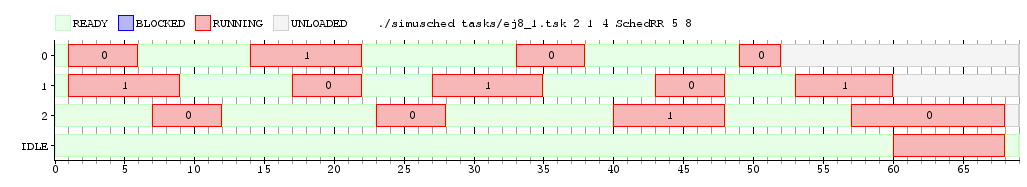
\includegraphics[width=1\columnwidth]{imagenes/ej8_1_rr.png}
        \caption{Escenario 1 en \emph{scheduler} con migración (\texttt{SchedRR})}
    \end{center}
\end{figure}

\begin{figure}[H]
    \begin{center}
        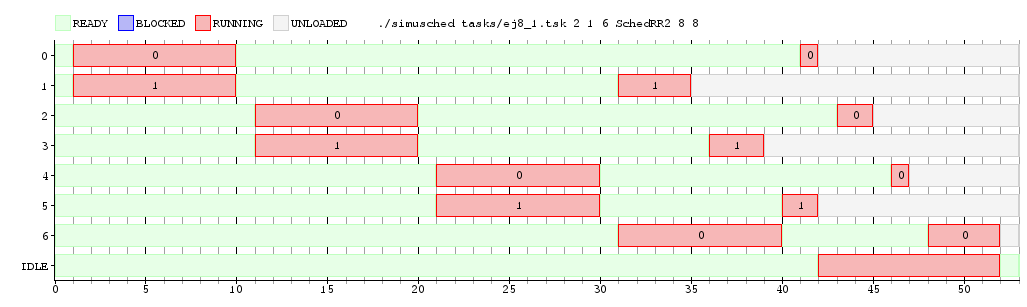
\includegraphics[width=1\columnwidth]{imagenes/ej8_1_rr2.png}
        \caption{Escenario 1 en \emph{scheduler} sin migración (\texttt{SchedRR2})}
    \end{center}
\end{figure}

\begin{figure}[H]
    \begin{center}
        \begin{tabular}{|c|c|c|c|}
            \hline
            \textbf{Scheduler} & \textbf{Waiting-time} & \textbf{Turnaround} \\ \hline
            \texttt{SchedRR}   & 32.333 & 60 \\
            \texttt{SchedRR2}  & 18.333 & 46 \\ \hline
        \end{tabular}
        \caption{Tiempos promedio para el Escenario 1, para cada \emph{scheduler}}
    \end{center}
\end{figure}


\begin{figure}[H]
    \begin{center}
        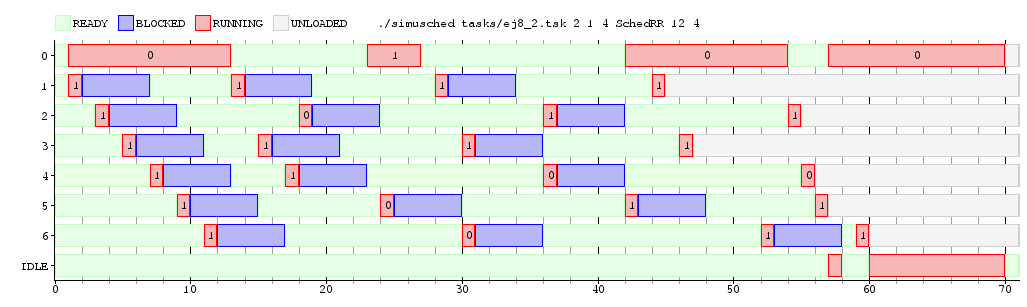
\includegraphics[width=1\columnwidth]{imagenes/ej8_2_rr.png}
        \caption{Escenario 2 en \emph{scheduler} con migración (\texttt{SchedRR})}
    \end{center}
\end{figure}

\begin{figure}[H]
    \begin{center}
        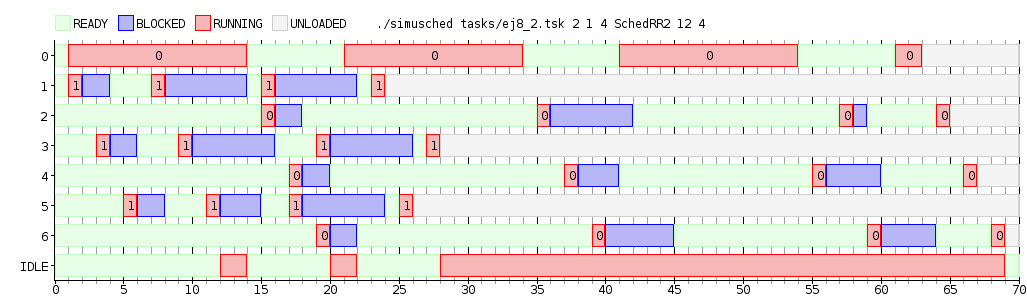
\includegraphics[width=1\columnwidth]{imagenes/ej8_2_rr2.png}
        \caption{Escenario 2 en \emph{scheduler} sin migración (\texttt{SchedRR2})}
    \end{center}
\end{figure}

\begin{figure}[H]
    \begin{center}
        \begin{tabular}{|c|c|c|c|}
            \hline
            \textbf{Scheduler} & \textbf{Latencia} & \textbf{Waiting-time} \\ \hline
            \texttt{SchedRR}   & 5.286 &  \\
            \texttt{SchedRR2}  & 8.714 &  \\ \hline
        \end{tabular}
        \caption{Tiempos promedio para el Escenario 2, para cada \emph{scheduler}}
    \end{center}
\end{figure}
